\documentclass{beamer}
\usepackage{graphicx}

\mode<presentation> {
%  \usetheme{Montpellier}
  \usecolortheme{beaver}
  \usecolortheme{orchid}
  \useoutertheme{tree}
  \useinnertheme{rounded}

  \setbeamercovered{transparent}
  % ou autre chose (il est �galement possible de supprimer cette ligne)
}

% Large and black subsection header at the top of the page
\setbeamerfont*{subsection in head/foot}{size=\large}
\setbeamercolor{subsection in head/foot}{fg=black}

\setlength{\parskip}{.3\baselineskip} 

%\usepackage[french]{babel}
\usepackage[latin1]{inputenc}
%\usepackage{times}
%\usepackage[T1]{fontenc}
% Or autre. Notez que le codage et la fonte doivent �tre assortis. Si T1
% ne para�t pas tr�s esth�tique, essayer d'effacer la ligne contenant fontenc.

\title % (facultatif, � utiliser uniquement si le titre de l'article est trop long)
{Thomson computers}

\subtitle {The history of Thomson 8-bit computers in France}

\author[] % (facultatif, � utiliser seulement avec plusieurs auteurs)
{Adrien Destugues - PulkoMandy}
% - Composez les noms dans l'ordre dans lequel ils appara�trons dans l'article
% - Utilisez la commande \inst{?} uniquement si les auteurs ont des affiliations
%   diff�rentes.

\institute[Forever 2016] % (facultatif mais g�n�ralement n�cessaire)
{
	Forever Party 2015 - Defender of the 8-bits
}
% - Utilisez la commande \inst uniquement s'il y a plusieurs affectations
% - Fa�tes quelque chose de simple, personne ne s'int�resse � votre adresse.

%\date % (facultatif)
%{6 juin 2009}

%\pgfdeclareimage[height=0.5cm]{le-logo}{haiku.pdf}
%\logo{\pgfuseimage{le-logo}}

% ne pas afficher les sous-sections dans la table des mati�res
\setcounter{tocdepth}{1}

% � supprimer si vous ne voulez pas que la table des mati�res apparaisse
% au d�but de chaque sous-section :
\AtBeginSection[] {
  \begin{frame}<beamer>{Plan}
    \tableofcontents[currentsection]
  \end{frame}
}

% Si vous souhaitez recouvrir vos transparents un � un,
% utilisez la commande suivante (pour plus d'info, voir la page 74 du manuel
% d'utilisation de Beamer (version 3.06) par Till Tantau) :
%\beamerdefaultoverlayspecification{<+->}

% Red�finir la page de titre (sans date dessus)
\defbeamertemplate*{title page}{progressbar theme}{
  \makeatletter
  \begin{center}
    \textbf{\textcolor{structure.fg}\large\inserttitle}

	\insertsubtitle
    
    \vskip\baselineskip
    \footnotesize\insertauthor\\[\baselineskip]
    \ifx\insertinstitute\@empty \else\tiny\insertinstitute\\[\baselineskip]\fi
  \end{center}
  \makeatother
}

\begin{document}

% Remove stupid "Figure:" label on picture captions
\setbeamertemplate{caption}{\raggedright\insertcaption\par}

\begin{frame}
  \titlepage
\end{frame}

\frame{
	\frametitle{Plan}
	\tableofcontents
}
  % Vous pouvez, si vous le souhaiter ajouter l'option [pausesections]

\section{History}
	\subsection{Thomson company}
		\begin{frame}
			The birth of Thomson
			\begin{itemize}
				\item 1879: Thomson-Houston company created in the USA
				\item 1892: Companie Fran�aise Thomson-Houston
				\item 1892: Merges with General Electric
			\end{itemize}
			The French company (CFTH) turns out to be not so useful to General
			Electric. It gradually becomes independant.

			
\includegraphics[width=.3\textwidth]{thomson-logo.jpg}
			
\includegraphics[width=.3\textwidth]{logo.png}
			
\includegraphics[width=.3\textwidth]{stmicro.jpg}

			
\includegraphics[width=.3\textwidth]{thomson-logo-0.jpg}
			
\includegraphics[width=.3\textwidth]{thmicro.jpg}

		\end{frame}

		\begin{frame}
			During the XXth century,
			Thomson buys other companies, gets too big, is split into several
			sub companies, some of which merge again.
			\begin{itemize}
				\item 1966: Thomson is split in Thomson-Brandt and Thomson-CSF
				\item 1981: Thomson-Brandt and Thomson-CSF are nationalized and merged again.
			\end{itemize}

			The nationalization happens because Thomson is a major supplier of
			weapons and high-tech devices for the French army (including
			semiconductors and other electronics related products). The French
			government doesn't want to rely on supplies of those coming from
			other countries, and wants to secure the local production.
		\end{frame}
	
		\begin{frame}
			Activities in various sectors over the XXth century:
			\begin{itemize}
				\item Electricity transport and production
				\item Tramways and Railways (will become ALSTOM)
				\item Batteries and Lightbulbs (Mazda)
				\item Weapons (Hotchkiss)
				\item Home appliances (Brandt)
				\item Semiconductors (EFCIS, will become ST microelectronics)
				\item Cathodic ray tubes and monitors
				\item ... and more (Technicolor, Thales, ...)
			\end{itemize}

			Thomson is involved in research about Radars, Magnetron, Videodiscs,
			the first "Eurovision" TV transmission, and much more.
		\end{frame}
	\subsection{Economics in France}
		\begin{frame}
			France is worried that the USA will take over the country
			\begin{itemize}
				\item This dates from WWII, mostly
				\item Politics and Economics are designed to avoid this
				\item Avoiding the use of English as much as possible
			\end{itemize}
		\end{frame}

		\begin{frame}
		The big US companies (Commodore, Apple, Atari and others) don't get to
		the French market as easily as elsewhere in Europe.
		\begin{itemize}
			\item High import taxes
			\item No easy way to setup a French subcompany (like Commodore Germany)
			\item French specific standards: SECAM, AZERTY, SCART (computers have to be modified to work with this)
		\end{itemize}
		\end{frame}
	\subsection{Computers in France}
		\begin{frame}
		This makes it easier for French companies to do their own computers
			\begin{itemize}
				\item Matra licences the MC10 design from Tandy and makes a French version of it
				\item Exelvision designs a computer using TI hardware
				\item Thomson builds theirs using Motorola 68xx family
				\item And much more (SMT, L�anord, LogAbax, Bull, ...)
			\end{itemize}
		\end{frame}

	\subsection{Plan Informatique Pour Tous}
		\begin{frame}
			"Informatique Pour Tous" - Computers for everyone!

		\begin{columns}[T]
			\begin{column}{.4\textwidth}
				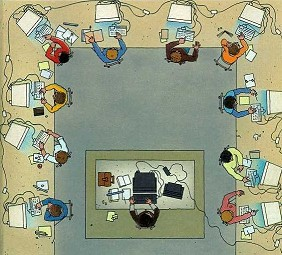
\includegraphics[width=\textwidth]{nanoreseau.jpg}
			\end{column}

			\begin{column}{.6\textwidth}
				\begin{itemize}
					\item French government plan to install computers in classrooms (6-15 year old children)
					\item Technical constraints enforcing a French manufacturer (SCART connector, LSEG language)
					\item Thomson will make most of the machines for this
				\end{itemize}
			\end{column}
		\end{columns}
		\end{frame}


		\begin{frame}
			Thomson solution
				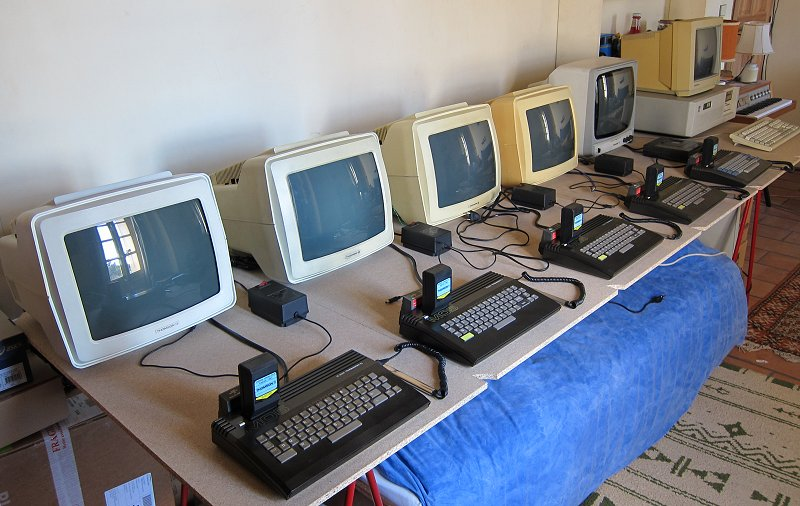
\includegraphics[width=.8\textwidth]{nanoreseau_01.jpg}

			\begin{itemize}
			\item "Student" computers: MO5 with RAM expansion and network interface
			\item The network is L�anord's Nanor�seau (RS485 based)
			\item "Teacher" computer (file server): Bull, LogAbax or SMT machines.
			\end{itemize}
		\end{frame}


\section{Timeline of Thomson computers}
	\subsection{General information}
		\begin{frame}
			\begin{itemize}
			\item All machines built around the 6809E CPU at 1MHz
			\item Video memory is made of two 8K pages
			\item No compatibility with anything else!

		The 6809E (and other Motorola chips) was already manufactured by Thomson-EFCIS
		for the French army, under license from Motorola. The 68xx chipset will be
		a popular one for French computers because of this (including Matra Alice,
		Tavernier, Apollo 7 Squale shown below).
			\end{itemize}

		\begin{columns}[T]
			\begin{column}{.3\textwidth}
				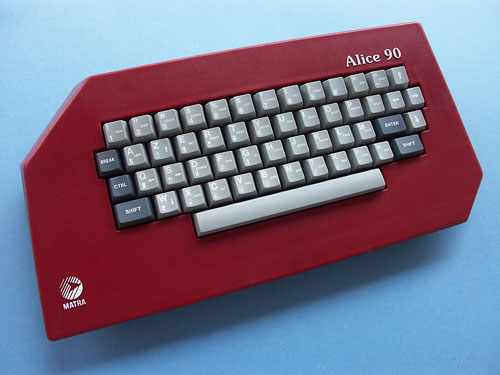
\includegraphics[width=\textwidth]{alice.jpg}
			\end{column}
			\begin{column}{.3\textwidth}
				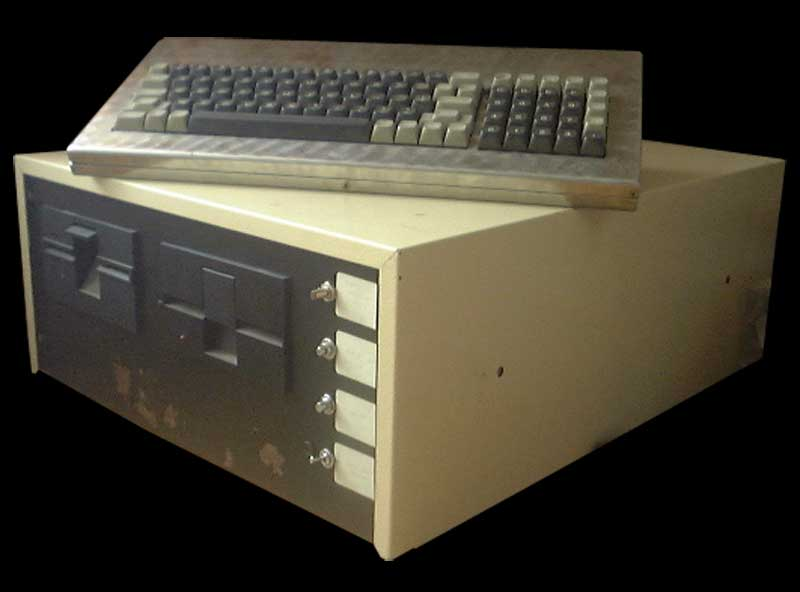
\includegraphics[width=\textwidth]{Tavernier.jpg}
			\end{column}
			\begin{column}{.3\textwidth}
				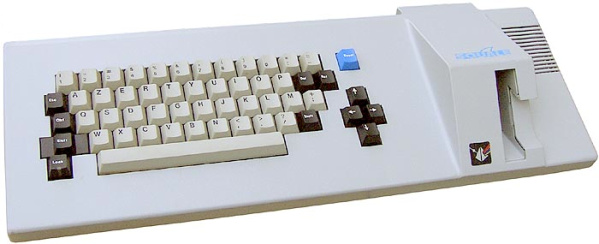
\includegraphics[width=\textwidth]{squale.jpg}
			\end{column}
		\end{columns}
		\end{frame}

	\subsection{Early design: the T9000 prototype}
		\begin{frame}
		Most of the design for the first machine is the work of Jos� Henrard.
		Researcher in sociology and economy, he built his own computer in his spare time and was then hired by Thomson to get the company started with computers.

		\begin{columns}[T]
			\begin{column}{.5\textwidth}
				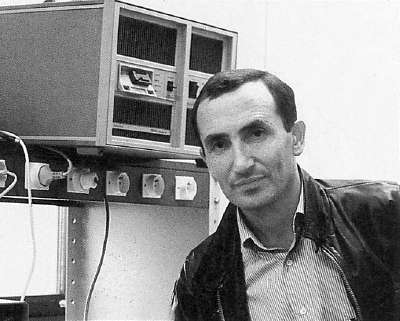
\includegraphics[width=\textwidth]{SiHenrard.jpg}
			\end{column}
			\begin{column}{.5\textwidth}
				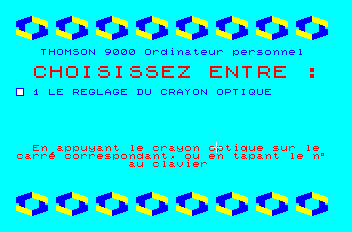
\includegraphics[width=\textwidth]{title-t9000.png}
			\end{column}
		\end{columns}


		This leads to the prototype T9000 computer demonstrated in 1979, a design
		very close to the TO7. Works then begin on industrializing the design.
		\end{frame}

	\subsection{TO7}
		\begin{frame}
		The TO7 is introduced in 1982. It competes against the Apple II and the zx81.

		"TO" means "T�l�vision Ordinateur", or "TV Computer", as it plugs to a standard TV.

		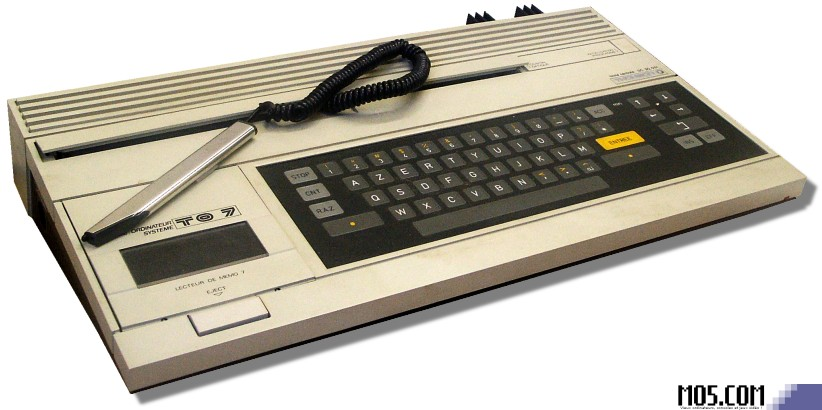
\includegraphics[width=\textwidth]{F_TO7.jpg}
		\end{frame}

		\begin{frame}
			Almost 24K of RAM:
			\begin{itemize}
				\item 8K system RAM (8 bits wide, expansion available to add 32K more),
				\item 8K video RAM (14 bits wide)
			\end{itemize}

			6K of ROM (built into the 6846 PIA):
			\begin{itemize}
				\item monitor code and "welcome" boot screen
				\item (BASIC comes in a cartridge, sold separately)
			\end{itemize}

		Static RAM is used, allowing a simple video generation system using standard 74LS logic chips.

		The computer is designed to be used mostly with the integrated lightpen.
		The keyboard is considered secondary and made flat in an attempt to make it less visible.
		\end{frame}

		\begin{frame}
		320x200, 8 color, with 8x1 color blocks, 2 colors per block.
		\begin{columns}[T]
			\begin{column}{.5\textwidth}
				\begin{figure}
				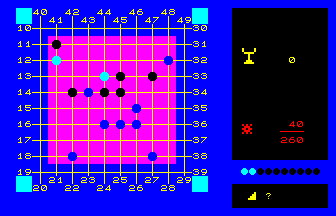
\includegraphics[width=\textwidth]{03.png}
				\caption{Atomium, 1982}
			\end{figure}
			\end{column}
			\begin{column}{.5\textwidth}
				\begin{figure}
				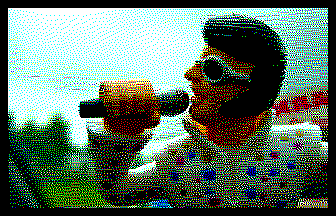
\includegraphics[width=\textwidth]{24.png}
				\caption{Elvis Lives! Slideshow, 2014}
			\end{figure}
			\end{column}
		\end{columns}
		Sound: 1-bit buzzer.
		\end{frame}

	\subsection{TO7/70}
		\begin{frame}
			Introduced in 1984, this competes against the Amstrad CPC 464 and Commodore 64.
			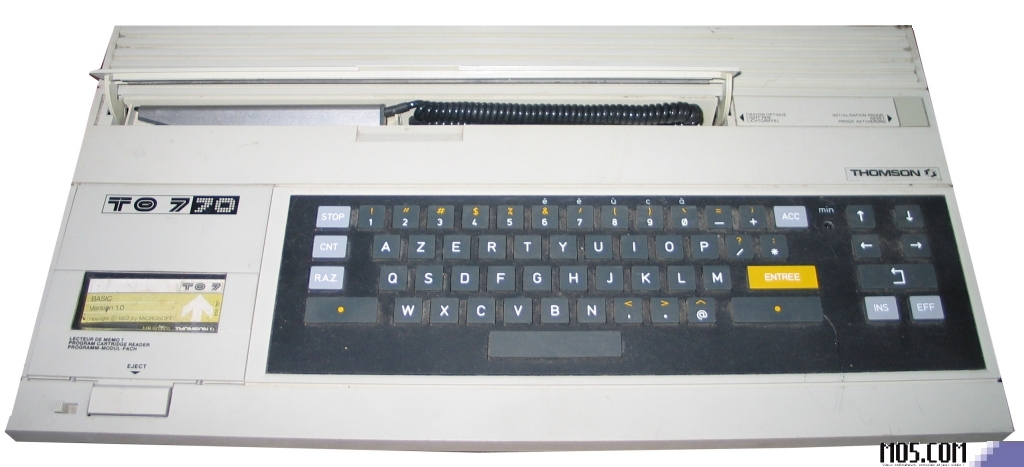
\includegraphics[width=\textwidth]{F_to770-2.jpg}

			64K RAM (48K system + 16K video), extensible to 128K.

			Dynamic RAM and integrated Gate Array for video logic.

			Slightly better "chicklet" keyboard.
		\end{frame}
		\begin{frame}
			The color palette has the 8 base colors, and brighter versions (not darker as on Spectrum).

			"bright white" is replaced with orange.
			\begin{figure}
		\begin{columns}[T]
			\begin{column}{.5\textwidth}
				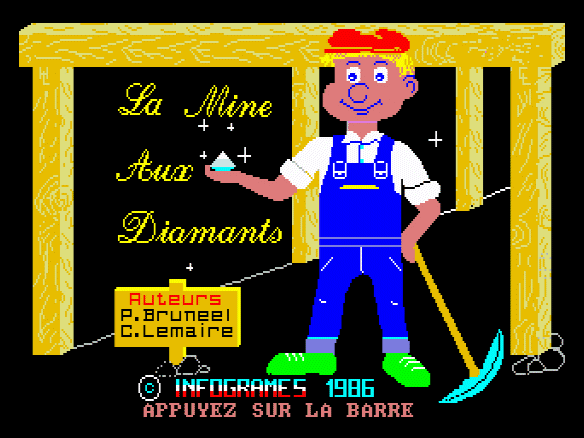
\includegraphics[width=\textwidth]{MOD1.png}
			\end{column}
			\begin{column}{.5\textwidth}
				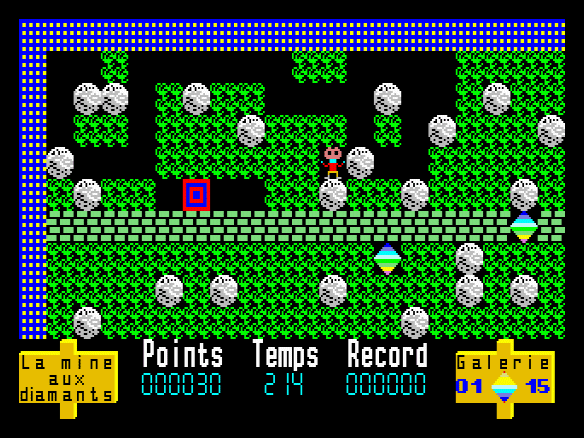
\includegraphics[width=\textwidth]{MOD2.png}
			\end{column}
		\end{columns}
				\caption{La mine aux diamants, 1984}
			\end{figure}
		\end{frame}

	\subsection{MO5}
		\begin{frame}
			The MO5 was launched at the same time as the TO7/70. It is a simpler design and competes against the ZX Spectrum and Oric Atmos.

				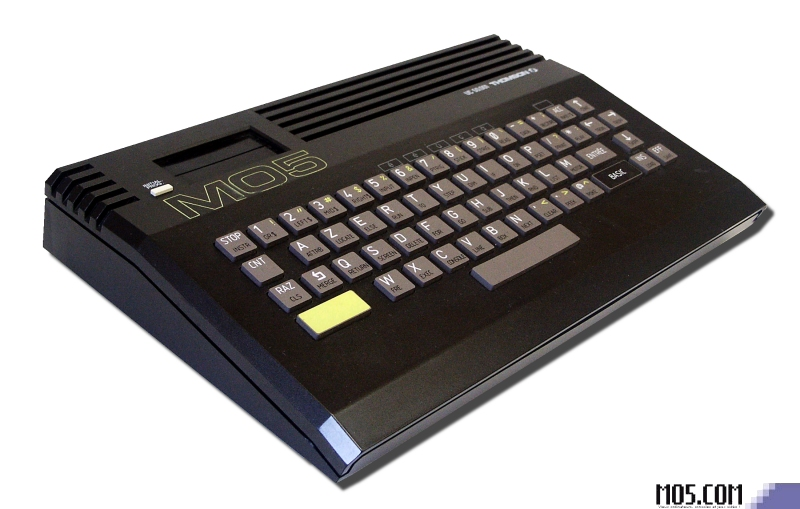
\includegraphics[width=\textwidth]{F_mo5.jpg}
		\end{frame}

		\begin{frame}
		\begin{columns}[T]
			\begin{column}{.04\textwidth}
				
\includegraphics[angle=90,width=\textwidth]{mo5pal.png}
			\end{column}
			\begin{column}{.96\textwidth}
			6846 PIA removed
			
			Simpler memory map with 16K ROM and 48K RAM
			
			Better tape data encoding.

			Built-in BASIC, masked by cartridges.

			No memory expansion initially, but fixed later to allow a 64K expansion on the cartridge port.

		\begin{columns}[T]
			\begin{column}{.5\textwidth}
			\begin{figure}
			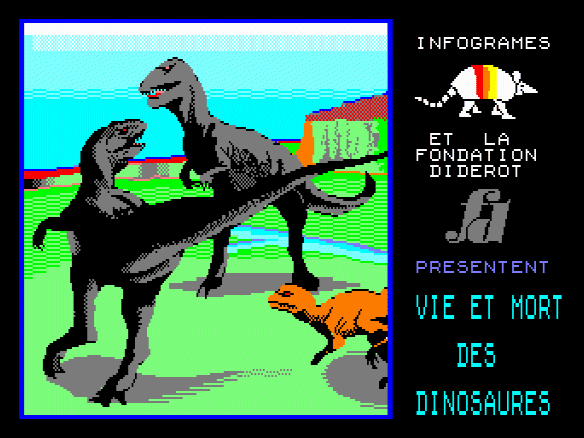
\includegraphics[width=\textwidth]{dinos.png}
			\caption{Life and death of Dinosaurs, 1986}
			\end{figure}
			\end{column}
			\begin{column}{.5\textwidth}
			\begin{figure}
			
\includegraphics[width=\textwidth]{poiscmo5.png}
			\caption{Poisca�e by Exocet, 2015}
			\end{figure}
			\end{column}
		\end{columns}


			
			\end{column}
		\end{columns}
		\end{frame}

	\subsection{TO9}
		\begin{frame}

		\begin{columns}[T]
			\begin{column}{.6\textwidth}
				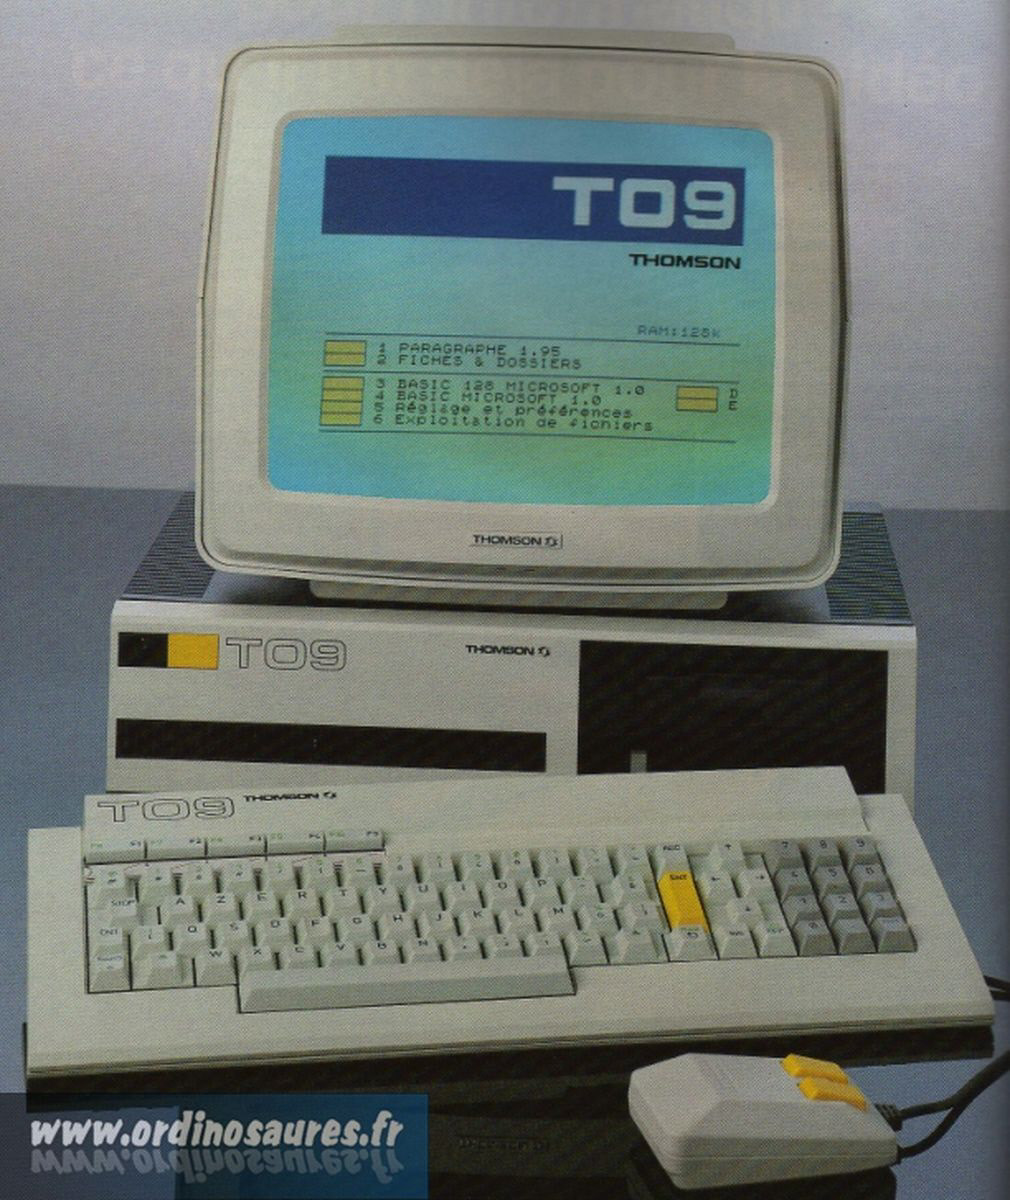
\includegraphics[width=\textwidth]{TO9.jpg}
			\end{column}

			\begin{column}{.4\textwidth}
				Introduced in 1985, the TO9 targets the professional market
			
				(competing against the Macintosh, according to Thomson marketing dept.)
			\end{column}
		\end{columns}
		\end{frame}

		\begin{frame}
			128K RAM, 136K ROM with built-in BASIC, Word processor, database, and "icon DOS" file manager.

			Built-in disk drive, PC like desktop case with detached keyboard

			6-bit DAC for sound output, Joystick/mouse ports, parallel port.

			(these are all available as expansion for other models).

			The same year, the TO7/70 and MO5 are upgraded to get a mechanical keyboard.

			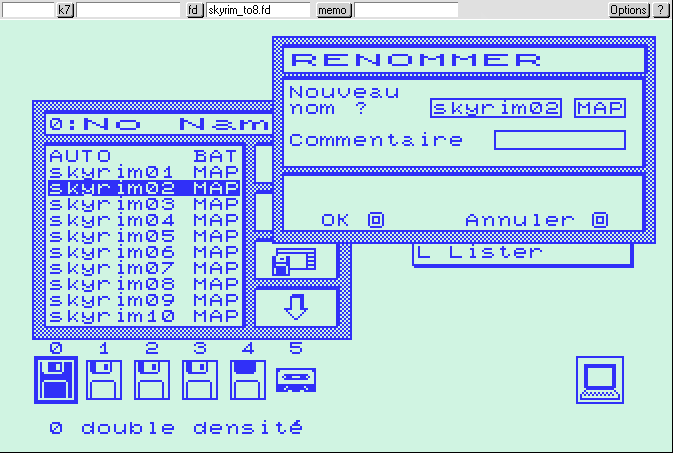
\includegraphics[width=.5\textwidth]{screenshot1.png}
		\end{frame}

		\begin{frame}
		\begin{columns}[T]
			\begin{column}{.7\textwidth}
			New video modes without block constraints
			
			(320x200 4 colors, 160x200 16 colors,
			
			640x200 2 colors)

			4096 color configurable palette.

				\begin{figure}
				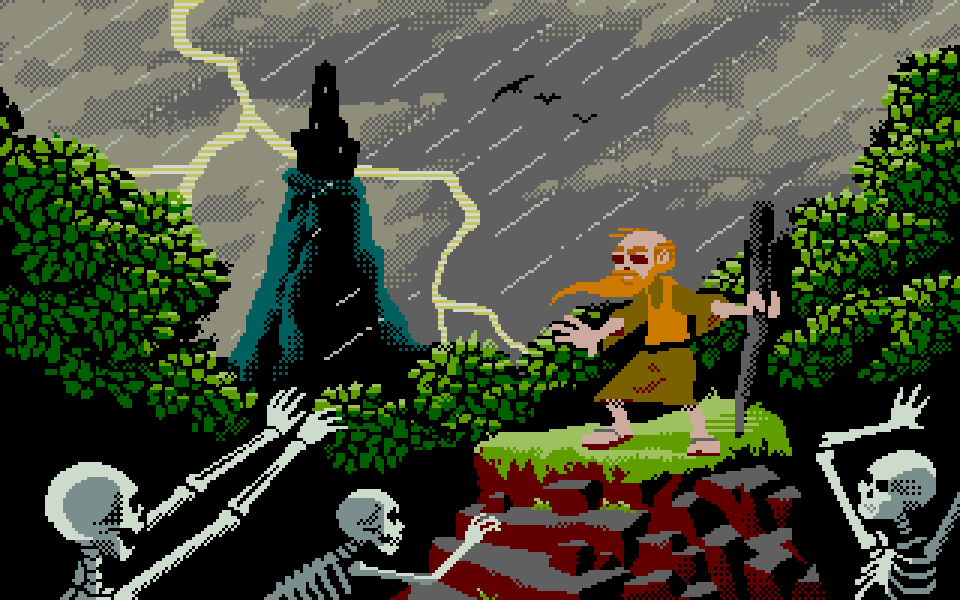
\includegraphics[width=\textwidth]{brink-thedruid.png}
				\caption{The Druid by Brink, 2014}
			\end{figure}
			\end{column}
			\begin{column}{.4\textwidth}
				\vspace{-.5cm}
				\begin{figure}
				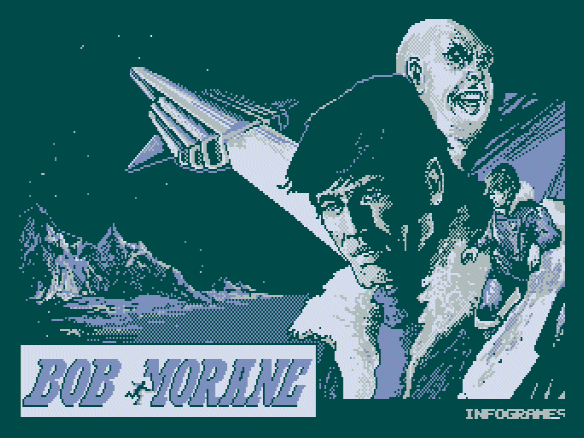
\includegraphics[width=\textwidth]{bob.png}
				\caption{Bob Morane Science Fiction}

				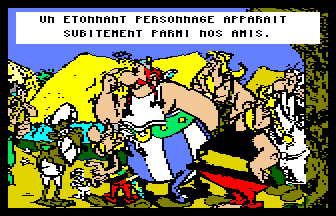
\includegraphics[width=\textwidth]{asterix.png}
				\caption{Asterix Chez Rahazade}
				\end{figure}
			\end{column}
		\end{columns}
		\end{frame}

	\subsection{The 1986 machines}
		\begin{frame}
			New gate array integrating more of the computer on a single chip to reduce costs.

			All the new features from the TO9 are made available on all machines.

			The ROM is 64K on MO6 and 80K on TO machines. The built-in software is now moved to floppies
			to allow easier upgrades (the first 10000 TO9 shipped had to be replaced because of software bugs).

		\end{frame}

		\begin{frame}
			The TO7/70 is replaced with the TO8 (now fighting against Amstrad CPC 6128, Amiga 500 and Atari ST),
			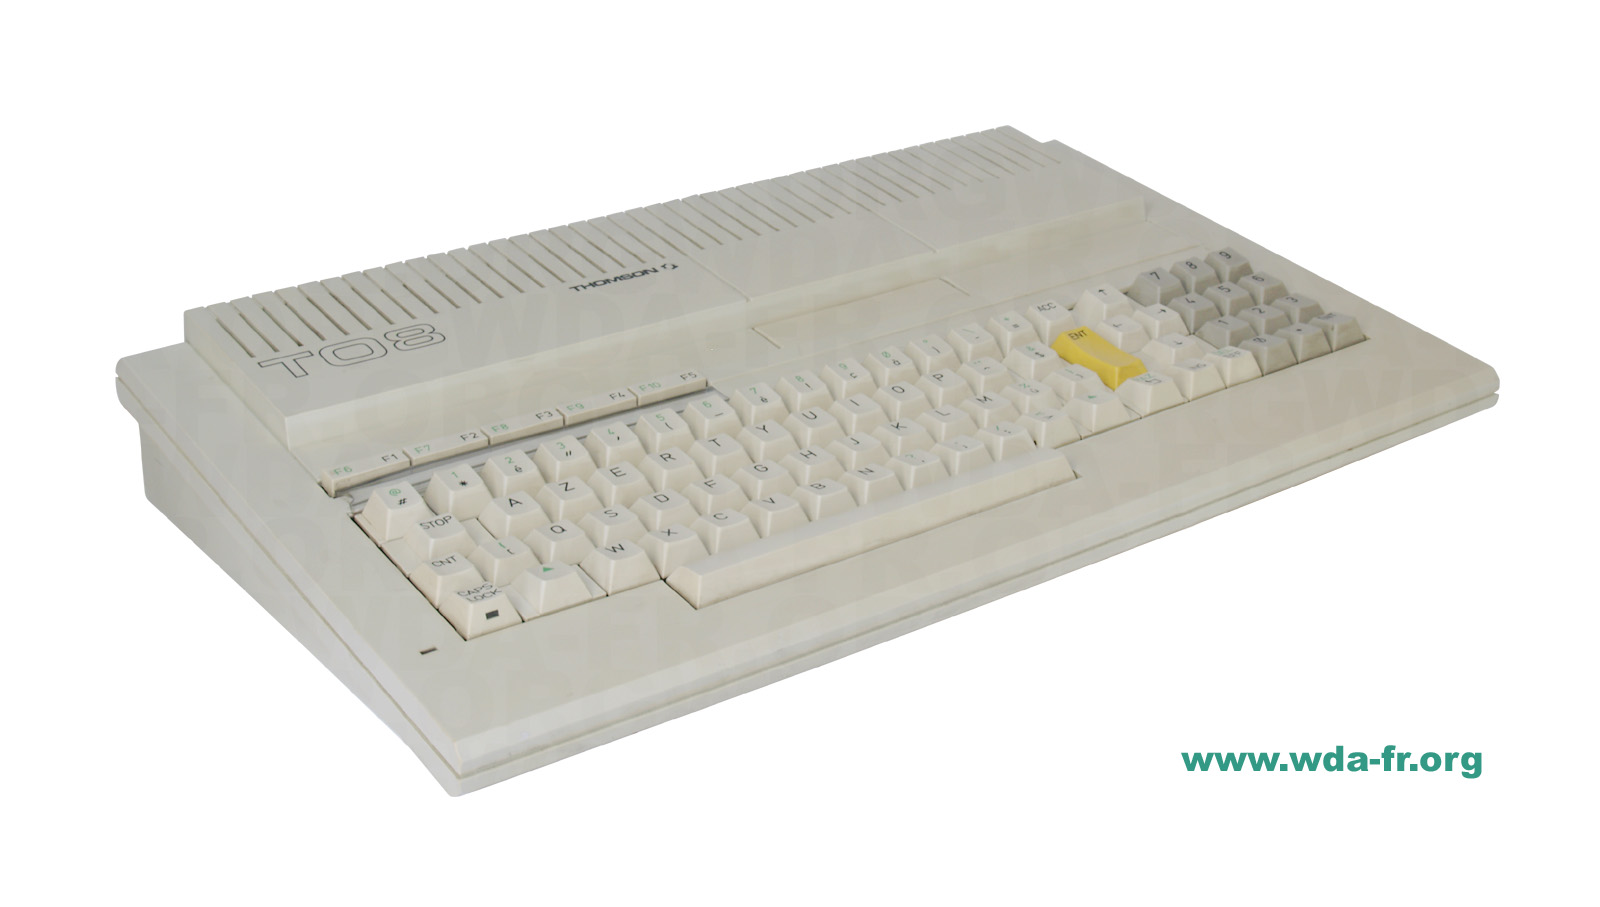
\includegraphics[width=\textwidth]{TO8.jpg}

			It gets an internal floppy controller and 256K RAM, but still no built-in floppy drive.
		\end{frame}

		\begin{frame}
			The MO5 is replaced with the MO6 (fighting against Amstrad CPC 464),
			which has 128K RAM and a built-in tape deck.

			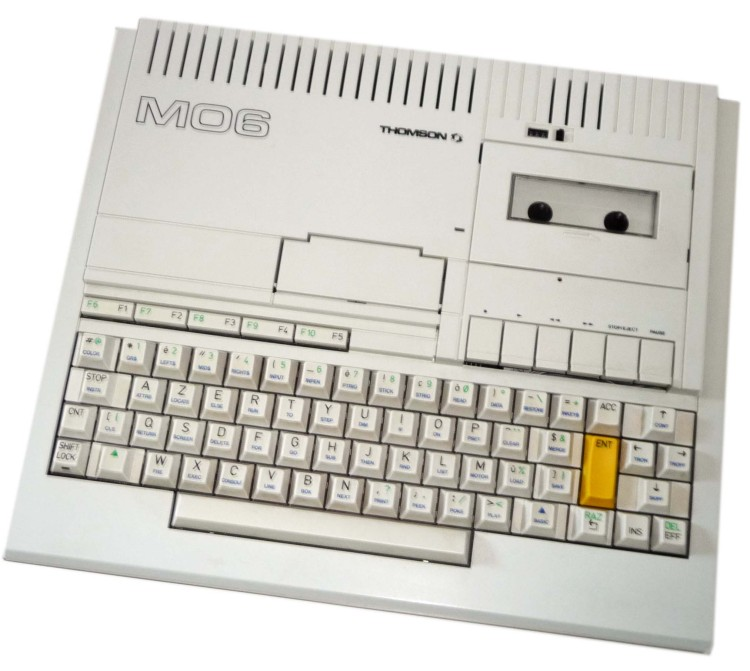
\includegraphics[width=\textwidth]{MO6.jpg}
		\end{frame}

		\begin{frame}
			The TO9 with the TO9+, getting 512K of RAM and a built-in modem.

			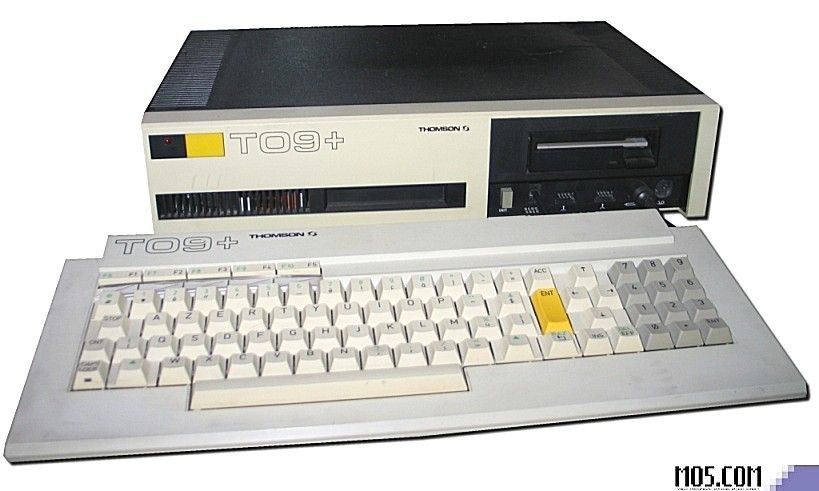
\includegraphics[width=\textwidth]{F_to9plus.jpg}
		\end{frame}

	\subsection{End of the story}
		\begin{frame}
			In 1987, the TO8 is replaced with the TO8D and finally gets a built-in floppy drive.

			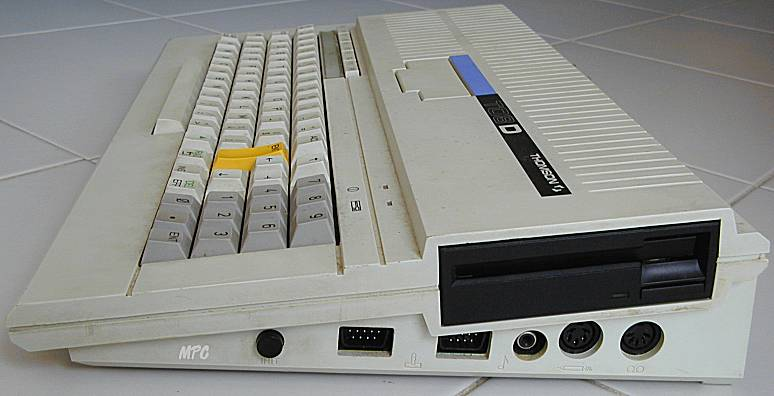
\includegraphics[width=\textwidth]{to8dcote.jpg}
		\end{frame}

		\begin{frame}
			Thomson teamed up with Olivetti (Italia) and Acorn (UK) to design an european standard computer.
			This was based on 68000 CPU and multitasking OS/9. The project is cancelled.

			Thomson will sell a PC compatible machine (the TO16) until 1989, then quit the microcomputer market.
		\end{frame}

\section{Programming on Thomson}
\subsection{The 6809E CPU}
	\begin{frame}
		\begin{itemize}
		\item Binary-incompatible redesign of the earlier 680x CPU
		\item Similar to the 6502, but more powerful
		\item 2 accumulators (A and B) useable as a 16-bit one (D)
		\item 2 index registers (X,Y)
		\item 2 stack pointers (S,U)
		\item Direct-page allows fast access to a 256-byte memory zone 
			(like Zero-page, but can use any 256-byte memory zone with DP register)
		\item Hardware mulitply instruction
		\item advanced addressing modes (indirect with predecrement/postincrement)
		\item LEA instruction (like on 68000)
		\end{itemize}
	\end{frame}

\subsection{Video logic}
	\begin{frame}
		Original design (1982-1985)
		\begin{itemize}
	\item The video hardware access the memory using a 16-bit bus 
	\item This is split in two "banks", the CPU can only map one at a time
	\item One bank sets 2 colors for a block (3 or 4bit each)
	\item The other bank defines the 8 pixels (0=use first color, 1=use second color)
	\item The resolution is fixed to 320x200, leaving a small free space in each bank
	\item Video memory is linear.
		\end{itemize}
	\end{frame}

	\begin{frame}
	Starting from the TO9, and in the 1986 gate array, some changes are made:
	\begin{itemize}
	\item The 4-bit colors are fed to a programmable lookup palette, allowing 4096 colors
	\item The pixel clock can be changed to generate 160x200 or 640x200 modes
	\item The "attribute block" system can be replaced by a planar or semi-planar mode (each pixel is defined using some bits from each bank)
	\item The system allows for "overprint" modes where one bank masks the other.
	\end{itemize}
	\end{frame}

	\begin{frame}
	In 1986, further changes are made:
	\begin{itemize}
	\item The memory access is done using the system 8-bit bus
	\item The two banks are interleaved in physical memory to allow "same-page" fast access
	\item This makes it possible to use a single bank of 8 256K chips for the whole memory
	\item As the Gate Array is also used on the MO6, an extra swapping step is added for compatibility.
	\end{itemize}
	
	\end{frame}

\subsection{Sound}
	\begin{frame}
	Up to the MO5, only a buzzer is available.

	Starting from the TO9, a 6-bit DAC is used. It has no DMA, so playing sound
	wastes a lot of CPU time, and some bits are shared with mouse input, which create interferences.

	Additionally, the tape drive has a stereo head. One track is used for data,
	and the other is sent to the audio amplifier. This can be used for CPU-free
	high-quality audio.
	\end{frame}

\subsection{Memory banking}
	\begin{frame}
		The ROM is always mapped in. This is why interrups are hardwired to it.

		On the MO5 and plain TO7, only the video RAM is banked (2 banks). But
		RAM expansions may add more.

		The TO9 adds even more banking support,

		The 1986 gate array is compatible with all of the above, and has yet another
		new mode to allow up to 512K of banks. It also allows relocating the video
		RAM to different memory banks instead of a single fixed one.

		Use of the different modes can be confusing. It's possible to map the same
		RAM page to the CPU at multiple places at a time.
	\end{frame}


\subsection{Extra features}
	\begin{frame}
		On TO machines, the 6846 PIA provides a programmable timer

		Unfortunately, the interrupt routine jumps into ROM, and does a lot of things
		there.

		You can still use the timer with polling, or the SYNC instruction to wait for
		timer events without using interrupts (but this of course locks the CPU waiting).
	\end{frame}

	\begin{frame}
		The 1986 gate array has 60Hz video support. This was never used, as attempts to export the machines have all failed (to URSS, India, Argentina, Spain, ...).

		This could be used to kill the bottom border of the screen like on Atari ST.

		The video modes are programmed using a 7-bit register. A lot of combinations are marked "useless" in the official documentation. What happens if you use them?
	\end{frame}


\section{Software failure}
\subsection{Why did it fail?}

\begin{frame}
As you probably have noticed, Thomson machines were never too popular out of
France. Why is that?
\begin{itemize}
	\item Too high prices: Thomson insisted on building the computers completely
		in France, and had somewhat complex hardware (lots of RAM and ROM, ...),
		leading to high prices.
	\item Too high compatibility: all machines use the same 1MHz CPU in an attempt to make them all compatible. In 1986,
		this was not acceptable anymore
	\item Too low compatibility: despite the attempts, there were still a lot of problems and misunderstandings (why keeping both the MO and TO series? Why replacing the Gate Array with a new and slightly different design in the MO5 later revisions?)
	\item Too many machines: and I only shown the ones with actual hardware differences, ignoring the various recasings (MO5NR, MO5 Platini, mechanical keyboard upgrades)
\end{itemize}
\end{frame}
\begin{frame}
\begin{itemize}
	\item Unusual CPU choice: Thomson and Tandy CoCo are the only ones using the 6809, forcing devs to use different tools and rewrite all their code. Z80 and 6502 were a lot more popular.
	\item Low quality software: most software is adapted from Spectrum or CPC,
		and not using Thomson machines capabilities to their full potential.
		Moreover, they kept compatibility with older models, and never used the
		advanced features of the new ones to the full power.
	\item "educative" orientation. Thomson is remembered for being the "school
		computer". It never managed to become a popular game machine, nor
		a business one.
\end{itemize}
\end{frame}

\subsection{Thomson demoscene}
\begin{frame}
In the 80s and 90s, there was an active Thomson community in France, but not
much demomaking activities. People focused mostly on writing "serious" software,
and some hardware projects.

In the 1990s, the only group was HCL. They did some intros as well as the HCL
megademo.

In the 2000s, the group PULS finally brings some serious demos to Thomson with
Chinese Stack and Space Project.

In 2011, for the forst time a Thomson demo enters a democompo (at Forever!)
\end{frame}

\section{Join us!}
\begin{frame}
I hope to see more people have a try at Thomson. You don't have one at home?
No problem, we have emulators!

Get MESS or TEO, both come with a built-in debugger and other useful features
for development.

Some of the hardware documentation is only available in French. (have a look at
the dcmoto website for some). I'm working on a "demomaker guide" to get you
started.

http://shinra.cpcscene.com
\end{frame}

\end{document}
